\subsection{\label{Contact}Bodies in Contact}

The method and functions described in this subsection require
{\bf contact/model2const.l, con\-tact/in\-e\-qual\-i\-ties.l,
 contact/drawconst.l}.

\begin{refdesc}

\classdesc{body}{object}{()}{defines a three dimensional shape.}

\methoddesc{:constraint}{b}{returns self's constraint
when self is in contact with {\em b}.}

\funcdesc{constrained-motion}{c}{returns the possible motions
which satisfy the constraint {\em c}.}

\funcdesc{constrained-force}{m}{returns the force which is applicable
from the constrained body to the constraining body.}

\funcdesc{draw-constraint}{c}{draws the constraint {\em c}.}

\funcdesc{draw-motion}{m a b}{draws the possible motions of {\em a}
in contact with {\em b}. Type the return key for drawing.}
\end{refdesc}
Example\\
\begin{verbatim}
;;
;;      peg in a hole with 6 contact points
;;
(in-package "GEOMETRY")
(load "view")
(load "../model2const.l" :package "GEOMETRY")
(load "../inequalities.l" :package "GEOMETRY")
(load "../drawconst.l" :package "GEOMETRY")

(setq x (make-prism '(#f(50 50 0) #f(50 -50 0) #f(-50 -50 0) #f(-50 50 0))
                    #f(0 0 200)))
(setq x1 (copy-object x))
(send x1 :translate #f(0 0 -100))
(send x1 :worldcoords)
(setq a1 (make-prism '(#f(100 100 -150) #f(100 -100 -150)
                       #f(-100 -100 -150) #f(-100 100 -150))
                     #f(0 0 150)))
(setq ana (body- a1 x1))
(send x :translate #f(0 -18.30127 -18.30127))
(send x :rotate -0.523599 :x)
(send x :worldcoords)

(setq c (list (send x :constraint ana)))
(setq m (constrained-motion c))
(setq f (constrained-force m))

(hidd x ana)
(draw-constraint c)
(draw-motion m)
\end{verbatim}
\clearpage
The following figures shows examples of constraints.
The small arrows in the figures designate the constraints for the pegs.
\\ 

\begin{figure}[h]
\includegraphics[width=7.9cm]{fig/fig-peg-in-hole1.ps}
%\epsfile{file=fig/fig-peg-in-hole1.ps,width=7.9cm}
%\mbox{
%\epsfxsize=7.5cm
%\epsfbox{fig/fig-peg-in-hole1.ps}
%}
\includegraphics[width=7.9cm]{fig/fig-peg-in-hole2.ps}
%\epsfile{file=fig/fig-peg-in-hole2.ps,width=7.9cm}\\
%\mbox{
%\epsfxsize=7.5cm
%\epsfbox{fig/fig-peg-in-hole2.ps}
%}
%\epsfile{file=fig/fig-peg-in-hole3.ps,width=7.9cm}
\includegraphics[width=7.9cm]{fig/fig-peg-in-hole3.ps}
%\mbox{
%\epsfxsize=7.5cm
%\epsfbox{fig/fig-peg-in-hole3.ps}
%}
%\epsfile{file=fig/fig-peg-in-hole4.ps,width=7.9cm}
\includegraphics[width=7.9cm]{fig/fig-peg-in-hole4.ps}
%\mbox{
%\epsfxsize=7.5cm
%\epsfbox{fig/fig-peg-in-hole4.ps}
%}
\caption{Constraints for a peg in a hole.}
\label{fig:peg-in-hole}
\end{figure}

\clearpage

The following figures shows an example of the possible motions
of a peg in a hole.
The example corresponds to the above program.\\

\begin{figure}[h]
\begin{center}
\includegraphics[width=7.9cm]{fig/fig-peg-naname-m1.ps}
%\epsfile{file=fig/fig-peg-naname-m1.ps,width=7.9cm}
%\mbox{
%\epsfxsize=7.5cm
%\epsfbox{fig/fig-peg-naname-m1.ps}
%}
%\epsfile{file=fig/fig-peg-naname-m2.ps,width=7.9cm}\\
\includegraphics[width=7.9cm]{fig/fig-peg-naname-m2.ps}
%\mbox{
%\epsfxsize=7.5cm
%\epsfbox{fig/fig-peg-naname-m2.ps}
%}
%\epsfile{file=fig/fig-peg-naname-m3.ps,width=7.9cm}
\includegraphics[width=7.9cm]{fig/fig-peg-naname-m3.ps}
%\mbox{
%\epsfxsize=7.5cm
%\epsfbox{fig/fig-peg-naname-m3.ps}
%}
%\epsfile{file=fig/fig-peg-naname-m4.ps,width=7.9cm}
\includegraphics[width=7.9cm]{fig/fig-peg-naname-m4.ps}
%\mbox{
%\epsfxsize=7.5cm
%\epsfbox{fig/fig-peg-naname-m4.ps}
%}
\end{center}
\caption{Possible motions of a peg in a hole}
\label{fig:peg-in-a-hole}
\end{figure}

\clearpage
